\documentclass[oneside,a4paper,12pt]{article}
\usepackage{graphicx}
\usepackage[section]{placeins}
\usepackage{listings}
\graphicspath{{~/templates/}, {../images/}}

\makeindex
\begin{document}
	\begin{titlepage}
		\includegraphics[width=4cm]{logopopo.png}
		\hspace*{\fill}
		\includegraphics[width=6cm]{univlille.png}
		
		\begin{center}
			\vspace{1cm}
			\textbf{TP RLI}\\
			\textbf{Réseau Modbus}\\
			\vspace{1cm}
			\textbf{Valentin DOSIAS, Maxence NEUS}\\
			\vspace{3cm}
			%\includegraphics[width=13cm]{titlepage.png}\\
			\vspace{\fill}
			\textbf{Novembre 2021}\\
		\end{center}
	\end{titlepage}
	
	\tableofcontents
	\newpage
	
	\section{Architecture}
	
	\begin{figure}[h]
		\centering
		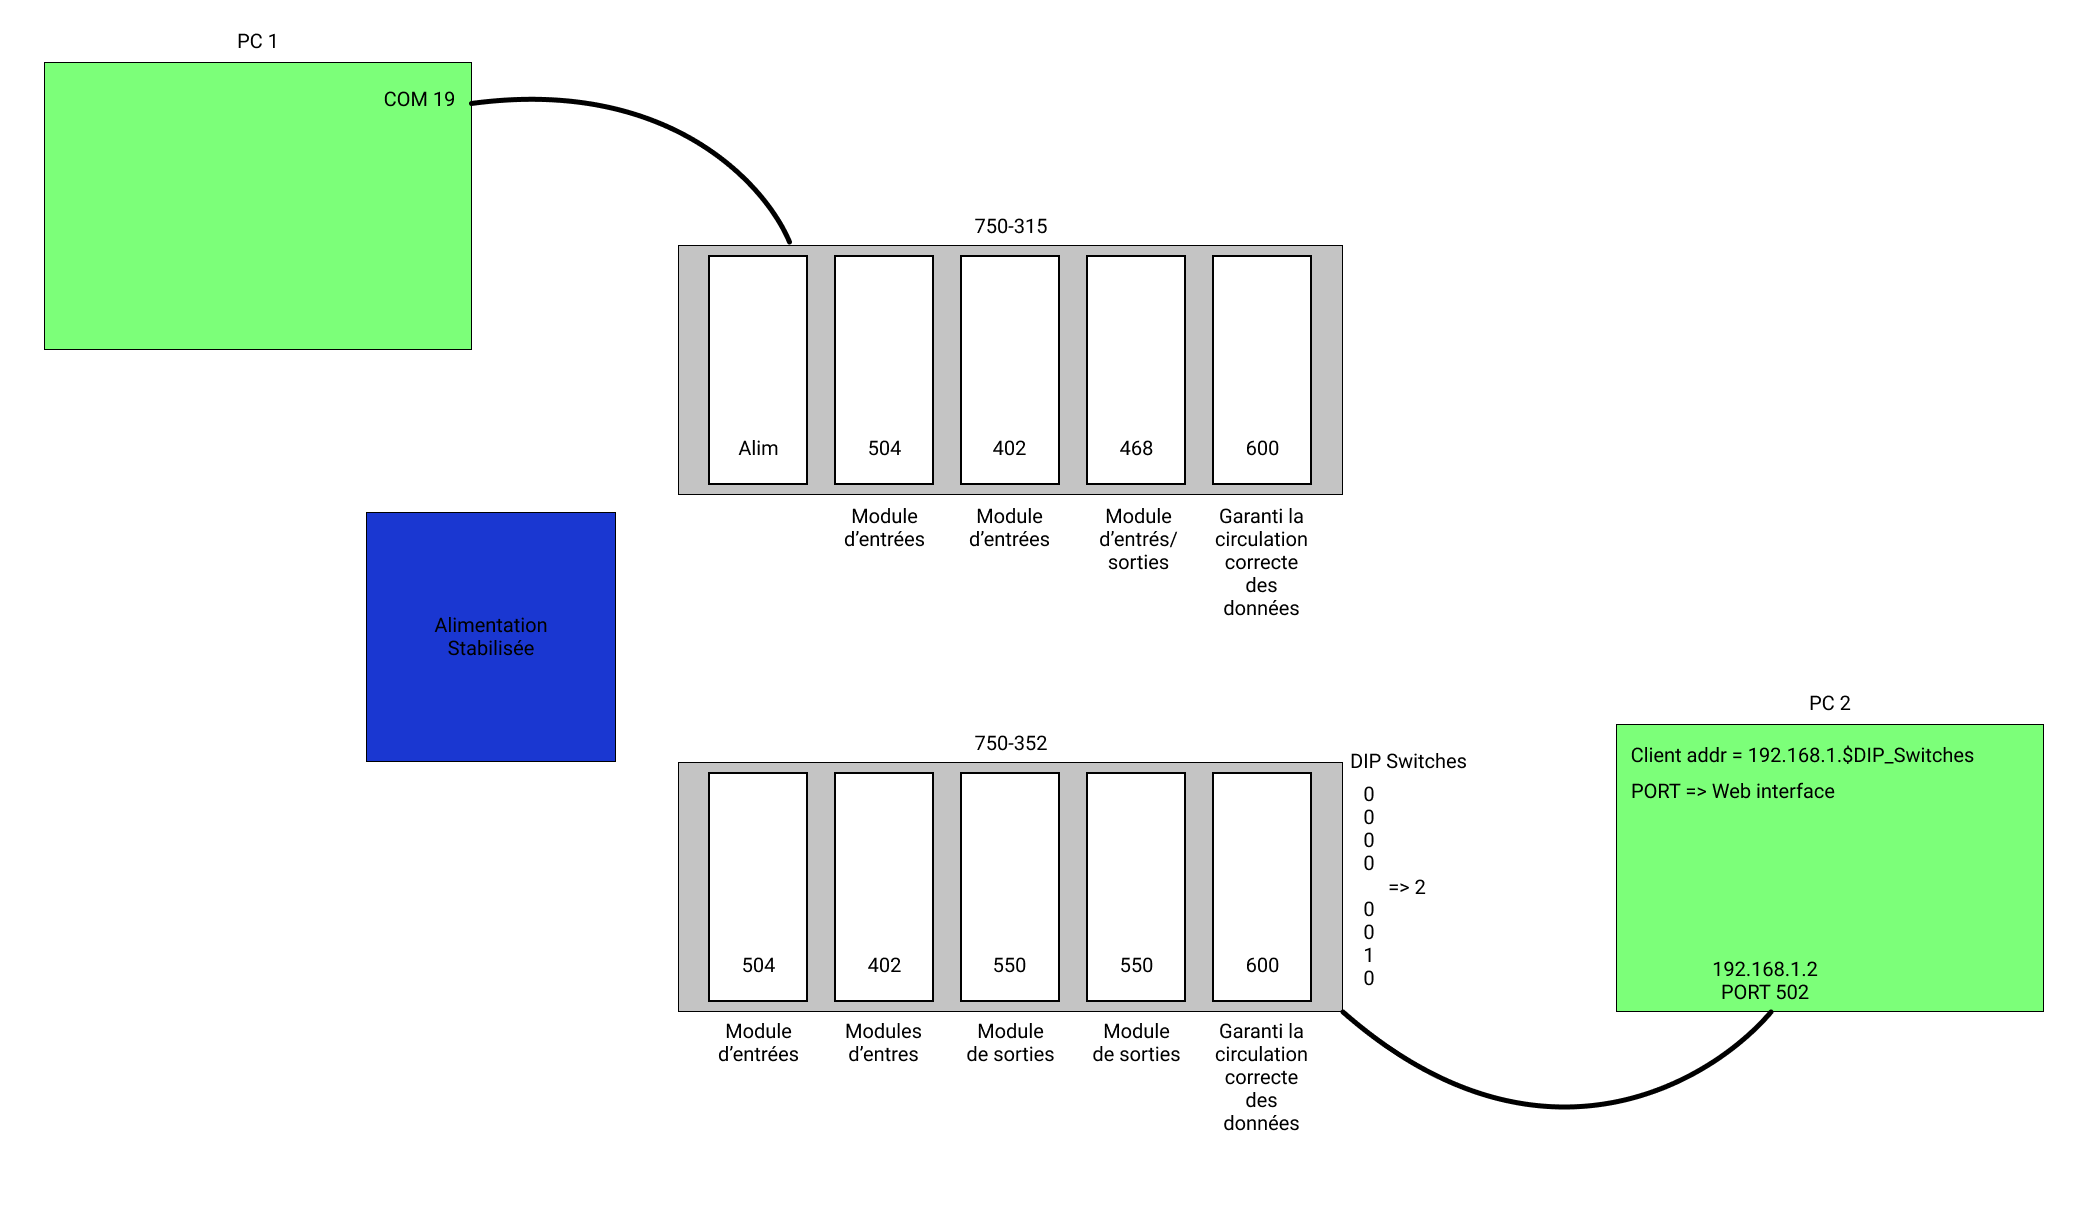
\includegraphics[width=14cm]{SchemaArchiRLI.png}
		\caption{Architecture}
	\end{figure}

	\section{Communication Modbus/TCP}
	
	Une fois connecté au module par la connexion ethernet, pour commander l'état des sorties, on doit envoyer une trame du type suivant :\\
	
	\begin{figure}[h]
		\begin{center}
			\begin{tabular}{|c|c|c|}
				\hline
				Champs & Valeur & notes\\
				\hline
				Transaction Identifier & 0x0000 & \\
				\hline
				Protocol Identifier & 0x0000 & \\
				\hline
				Length Field & 0x0006 & Longueur de la trame\\
				\hline
				Unit Identifier & 0x01 & pas utilisé\\
				\hline
				Function Code & 0x05 & Code de Write Coil (5)\\
				\hline
				Reference Number & 0x0001 &\\
				\hline
				ON/OFF & 0xFF & 0xFF=ON 0x00=OFF\\
				\hline
				& 0x00 & Fin de trame\\
				\hline
			\end{tabular}
		\end{center}
		\caption{Trame de Write Coil}
	\end{figure} 
	
	Pour la lecture des entrées, il faut envoyer une trame du type suivant :\\
	
	\begin{figure}[h]
		\begin{center}
			\begin{tabular}{|c|c|c|}
				\hline
				Champs & Valeur & notes\\
				\hline
				Transaction Identifier & 0x0000 & \\
				\hline
				Protocol Identifier & 0x0000 & \\
				\hline
				Length Field & 0x0006 & Longueur de la trame\\
				\hline
				Unit Identifier & 0x01 & pas utilisé\\
				\hline
				Function Code & 0x01 & Code de Read Coil (1)\\
				\hline
				Reference Number & 0x0001 &\\
				\hline
				Bit count & 0x0008 & Nombre de bits à aligner\\
				\hline
			\end{tabular}
		\end{center}
		\caption{Trame de Read Coil}
	\end{figure} 
	
	\section{Etude de la communication Modbus/RS485}
	
	\subsection{Evaluation du CRC}
	
	\begin{figure}[h]
	\begin{lstlisting}
uint16 CRC16(unsigned char message[], int lg) {
	uint16 crc = 0xFFFF;
	for (int pos=0; pos<lg;pos++) {
		crc^= = (UInt16)buf[pos];
		for (int i=8;i!=0;i--){
			if ((crc & 0xA001)) != 0)
			{crc>>=1;
				crc ^=0xA001;
			}
			else {crc>>=1}
		}
	}
	return crc;
}
	\end{lstlisting}
	\caption{Code de calcul du CRC}
	\end{figure}
	
	\subsection{Communiquer avec le boitier d'entrées/sorties}
	
	Pour communiquer avec le module, il faut déterminer l'addresse de l'esclave associée, pour cela, il suffit de lire sur l'appareil les valeurs des potentiomètres. Dans notre cas cette addresse est 0x02.\\
	
	Le CRC est à calculer à partir du début de la trame avec le code décrit plus haut. Il faut penser à inverser l'ordre des poids hauts et faibles dans la trame.\\
	
	\begin{figure}[h]
		\begin{center}
			\begin{tabular}{|c|c|c|}
				\hline
				Champs & Valeur & notes\\
				\hline
				Slave Address & 0x02 & Addresse de l'esclave\\
				\hline
				Function Code & 0x05 & Code de Force Single Coil\\
				\hline
				Coil address High/Low & 0x00 - 0x00 & Addresse de la sortie à commander\\
				\hline
				Force data High/Low & 0xFF - 0x00 & 0xFF00=ON, 0x0000=OFF\\
				\hline
				CRC Low & -- & \\
				\hline
				CRC High & -- & \\
				\hline
			\end{tabular}
		\end{center}
		\caption{Trame de Force Single Coil}
	\end{figure}
	
	\newpage
	\section{Commande d'un processus au travers de Modbus/RS485}
	
	Le fonctionnement du programme en général est tant que  le niveau bas de la cuve est à 0 on rempli la cuve jusqu'à ce que le niveau haut passe à 1.
\\
	On active le tapis tant que la bouteille n'est pas pleine.
\\
	On fait un versement rapide de 0 à 35 et de 35 à 50 un versement lent pour éviter les pertes.\\
	\begin{figure}[h]
		\centering
		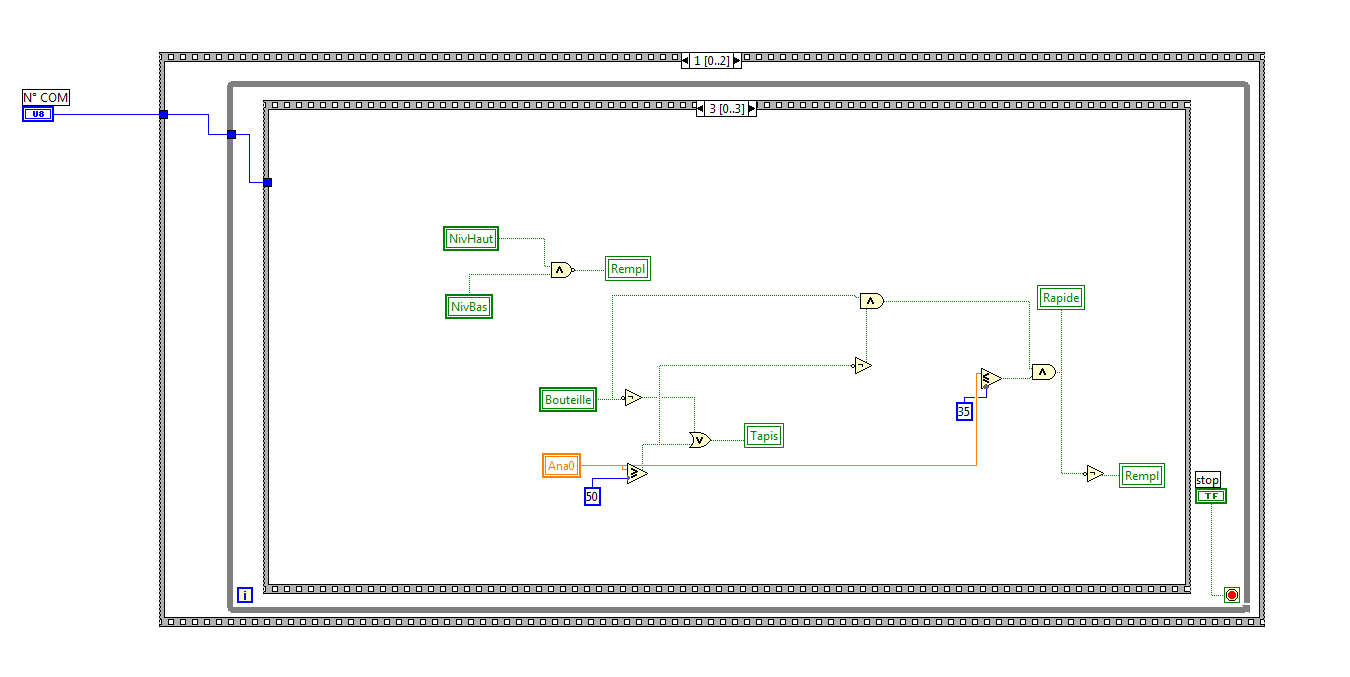
\includegraphics[width=16cm]{automatisation.png}
		\caption{Algorithme de remplissage}
	\end{figure}
	
	\section{Evaluation du temps de réponse}
	
\end{document}
